\documentclass[beleg,zihtitle,american,final,hyperref,utf8,oneside]{zihpub}

% Libraries
\usepackage{setspace}
\usepackage{booktabs} % for \toprule, \midrule, \bottomrule, \cmidrule
\usepackage{pgfplots}
\usetikzlibrary{positioning}
\usepackage{enumitem}
\pgfplotsset{compat=1.18}
\usepackage{siunitx}
\sisetup{
  per-mode = symbol,
  group-minimum-digits = 4,
  mode = match,
  reset-text-series = false,
  text-series-to-math = true,
  reset-text-family = false,
  text-family-to-math = true
}
\usepgfplotslibrary{groupplots,statistics,fillbetween,dateplot}
\newcommand{\BibLaTeX}{\textsc{Bib}\LaTeX}

\author{Benjamin-Elias Probst}
\title{Eigentokens: Grammar-Aware Inline Deduplication and Deterministic Compilation for Large Language Models}
\bibfiles{doku}

\birthday{11. April 1996}
\placeofbirth{Potsdam}
\matno{4510512}

\betreuer{Prof. Dr. Michael Färber}

\begin{document}

\let\cleardoublepage\clearpage
\selectlanguage{american} % ensure US English is active

% ---------------------------------------------------------
% ZOPP structure (headings only; content to be added later)
% ---------------------------------------------------------

% (Optional) Abstract
\chapter*{Abstract}
Eigentokens is a compilation-oriented view on language modelling: instead of treating a corpus as an opaque training set for gradient-descent optimisation, it treats \emph{deduplication, fingerprints, and grammars} as an intermediate representation that can be compiled into a usable model artifact.

This report describes \textbf{ComdareDB}, a database prototype that stores heterogeneous data, performs inline deduplication, and asynchronously infers grammar fragments from stored content. The work is guided by two research questions:

\begin{itemize}
  \item \textbf{RQ1:} Is it possible to compile a language model artifact (LLM-compatible in its interface) and subsequently use it efficiently?
  \item \textbf{RQ2:} What is grammar, and how can grammar be learned from real-world data in a context-sensitive way?
\end{itemize}

ComdareDB combines multi-fingerprint similarity search (exact hashes, rolling fingerprints, and locality-sensitive hashes) with a context-aware pointer graph over chunks. Background jobs refine deduplication decisions, infer grammar hypotheses, and emit a deterministic, traceable binary artifact, the \emph{Compiled Eigentoken Language Model (CELM)}. CELM does not aim to replace transformer-based LLMs; instead it provides \emph{traceable program output}: given an input string it returns similar chunks and their predecessors/successors, together with the grammar rules that justify these links.

The planned evaluation focuses on storage- and pipeline-level metrics (deduplication ratio, average in-/out-degree of chunk pointers, index write amplification, throughput and latency), and task-level indicators for retrieval and query compilation quality.
\chapter*{Project Context and Assignment}
% \addcontentsline{toc}{chapter}{Project Context and Assignment} % uncomment if desired

\noindent \textbf{Institution:} Faculty of Computer Science, Institute of Systems Architecture, Chair of Scalable Software Architectures for Data Analytics, Technische Universit\"at Dresden.

\noindent \textbf{Degree program:} Diploma in Computer Science (Pr\"ufungsordnung (PO) 2010).

\noindent \textbf{Module:} INF-PM-FPA Profilprojekt Anwendungsforschung in der Informatik.

\noindent \textbf{Work period:} 28.10.2025 -- 10.02.2026 (15 weeks).

\noindent \textbf{Supervision and reviewers:}
\begin{itemize}
  \item Supervising professor and supervisor: Prof. Dr. Michael F\"arber
  \item First reviewer: Prof. Dr. Michael F\"arber
  \item Second reviewer: n.\,n.
\end{itemize}

\noindent \textbf{Topic (condensed):} Eigentokens: grammar-aware inline deduplication and a deterministic compilation language for Eigentoken Language Model (ELM) / CELM-lang (CELM) artifacts, using a Secure Hash Algorithm 512-bit (SHA-512) indexed non-strict B\textsuperscript{+}-forest layout and an S3/key-value (KV) facade with Hypertext Transfer Protocol (HTTP) Range semantics (Request for Comments (RFC) 9110) \cite{Fielding2022}.

\noindent \textbf{Non-goals:} Natural Language Processing (NLP) tokenization and probabilistic inference/sampling are out of scope for the initial prototype.

\section*{Work Packages (Merged)}
\begin{itemize}
  \item \textbf{Requirements and scope:} use-cases, Service Level Objectives (SLOs), terminology; explicit non-goals; evaluation plan.
  \item \textbf{Architecture and specification:} Eigentoken tuple $\langle \mathit{id}, P, D, R \rangle$, grammar induction algorithm, non-strict B\textsuperscript{+}-forest with SHA-512, token/block mapping, RFC-9110 compliant Range mapping.
  \item \textbf{Core implementation (C++):} Grammar Induction Engine (A1), B\textsuperscript{+}-Forest Index (A2), Asynchronous Processing Pipeline (A3), S3/KV Interface (A4), Analysis and Control Application Programming Interface (API) (A5), Mock Rules and Testing Suite (A6).
  \item \textbf{CELM-lang integration:} M2-level meta-language for interpretation programs, pattern generators, match conditions, dynamic runtime extension; foundations for M3-level self-improvement routines.
  \item \textbf{Range path and optimization:} token-aligned block maps, heuristics for hot ranges, asynchronous consolidation.
  \item \textbf{Benchmarks and evaluation (incl. ablations):} datasets (code, text/logs, binary, and columnar formats), baselines, metrics (space, ingest, write/deletion amplification, percentiles P50/P95/P99), robustness under shift/insert/rename transformations.
  \item \textbf{Artifacts and reproducibility:} Command Line Interface (CLI), scripts, reproducible plots, report (\textasciitilde 20 pages), slide deck; scientific documentation and a colloquium presentation.
  \item \textbf{Roadmap (optional):} replication/erasure coding on grammar leaves; sketch the ELM/CELM compilation path for deterministic model generation.
\end{itemize}

\section*{Deliverables and Colloquium}
Submission includes: C++ prototype with CLI, benchmark scripts (and datasets/links), reproducible evaluations (plots), report (Portable Document Format (PDF)), and slide deck (PDF). The project concludes with a colloquium featuring a 60-minute talk and serves as preparation for the diploma thesis.


\chapter{Introduction and Motivation}
Large Language Models (LLMs) have become a standard building block for search, analytics, and software tooling. The dominant architecture is the Transformer \cite{Vaswani2017}, with decoder-only variants (GPT-style) trained via next-token prediction \cite{Brown2020}, encoder-only variants trained via masked language modelling (BERT) \cite{Devlin2018}, and encoder--decoder variants that treat every task as text-to-text (T5) \cite{Raffel2020}. At scale, many systems additionally rely on techniques such as Mixture-of-Experts for sparse scaling \cite{Shazeer2017,Fedus2021}, retrieval-augmented generation (RAG) \cite{Lewis2020}, and instruction tuning with human feedback (RLHF / InstructGPT) \cite{Ouyang2022}.

Despite this progress, the \emph{data-to-model pipeline} remains expensive and often opaque: training and fine-tuning require specialised hardware, the resulting knowledge is stored implicitly in weights, and it is hard to obtain traceable explanations of why a specific output was produced. In many practical settings, however, the desired behaviour is not creative generation but \textbf{auditable reuse of previously observed information} with strong provenance and predictable performance.

This work explores an alternative lens: \textbf{Eigentokens} treats a dataset as a graph of deduplicated chunks enriched by multiple fingerprints and contextual pointers. From this representation, ComdareDB infers grammar hypotheses that serve as an intermediate representation (IR). The IR can then be \emph{compiled} into a deterministic, executable artifact---a \emph{Compiled Eigentoken Language Model (CELM)}---whose output is traceable back to stored chunks and grammar rules.

\section{Research Questions and Scope}
This report focuses on the database side of the problem. The goal is \emph{not} to propose yet another neural backbone, but to show how a database can expose a compilation-grade representation of language and knowledge.

\begin{itemize}
  \item \textbf{RQ1:} Is it possible to compile a language model artifact (LLM-compatible in its interface) and subsequently use it efficiently?
  \item \textbf{RQ2:} What is grammar (in the sense of the Chomsky hierarchy), and how can grammar be learned from real-world data in a context-sensitive way?
\end{itemize}

\noindent The proof-of-concept is a fully functional database prototype with multiple storage interfaces and an analysis interface for real-time query of strings and metrics. A full benchmarking campaign is intentionally deferred to a later iteration; this document establishes the conceptual and architectural basis, plus an evaluation plan and metric definitions.

\section{Contributions}
The main contributions of this report are:
\begin{itemize}
  \item A database-centric architecture (ComdareDB) that combines inline deduplication, multi-fingerprint indexing, and a context-aware pointer graph over chunks.
  \item A description of an asynchronous pipeline that refines fingerprints and grammar hypotheses without blocking ingestion throughput.
  \item A compilation target (CELM) with a retrieval output contract that prioritises traceability and reproducibility over unconstrained generation.
  \item A set of evaluation metrics grounded in storage systems research (deduplication ratio, pointer graph statistics, index write amplification, throughput, and latency).
\end{itemize}
\chapter{Related Work and Background}
\section{Deduplication, Chunking, and Similarity Search}
Content-defined chunking (CDC) is a common approach for deduplication in storage systems because it is robust to insertions and shifts: a rolling fingerprint defines chunk boundaries, allowing similar regions to align even when byte offsets change \cite{Muthitacharoen2001,Eshghi2005}. Modern CDC variants such as FastCDC optimise throughput and boundary stability for practical deployments \cite{Xia2016}. Systems like Venti store blocks addressed by content hashes to provide archival storage with strong integrity guarantees \cite{Quinlan2002}.

While cryptographic hashes detect \emph{exact} duplicates, near-duplicate and cross-format similarity require additional signals. Locality-sensitive hashing (LSH) provides a principled way to perform approximate nearest-neighbour queries in high-dimensional spaces \cite{Indyk1998}. In practice, document resemblance can be approximated with MinHash \cite{Broder1997}, and compact similarity sketches can be built with SimHash \cite{Charikar2002}. These techniques motivate ComdareDB's \emph{multi-fingerprint} design: different fingerprints act as orthogonal ``lenses'' to find equivalent or related data and thus recover additional pieces of an emerging grammar.

\section{Grammar Induction and Grammar-Based Compression}
Grammar-based compression views a sequence as being generated by a grammar and aims to infer a compact set of production rules that reproduces the input. Sequitur incrementally infers a context-free grammar by introducing non-terminals for repeated digrams \cite{NevillManning1997}. Re-Pair similarly replaces the most frequent pair iteratively and is widely used as a simple grammar compressor \cite{Larsson2000}. These methods connect compression and structure discovery: repeated patterns become reusable rules, and the induced grammar can serve as a structured representation of the dataset.

\section{Mainstream LLM Systems and Techniques}
Modern LLM systems are largely built on the Transformer architecture \cite{Vaswani2017}. What differs across systems is the \emph{training objective}, the \emph{scaling strategy}, and the \emph{augmentation/finetuning techniques}. Table~\ref{tab:llm_reference_table} summarises representative model families and techniques with their primary references.

\begin{table}[ht]
\centering
\caption{Representative LLM families and techniques with primary references.}
\label{tab:llm_reference_table}
\begin{tabularx}{\textwidth}{>{\raggedright\arraybackslash}X l l >{\raggedright\arraybackslash}X}
\toprule
System / technique & Architecture & Objective / role & Primary reference \\
\midrule
Transformer (baseline) & encoder/decoder attention & general sequence modelling & \cite{Vaswani2017} \\
GPT-style LLMs & decoder-only Transformer & next-token prediction & \cite{Brown2020} \\
BERT & encoder-only Transformer & masked language modelling & \cite{Devlin2018} \\
T5 & encoder--decoder Transformer & text-to-text denoising & \cite{Raffel2020} \\
PaLM & large decoder-only Transformer & scaled next-token prediction & \cite{Chowdhery2022} \\
LLaMA & decoder-only Transformer & efficient foundation model training & \cite{Touvron2023} \\
Mixture-of-Experts (MoE) & sparse expert routing & scaling via sparsity & \cite{Shazeer2017,Fedus2021} \\
RAG & retriever + generator & grounding via retrieval & \cite{Lewis2020} \\
RLHF / InstructGPT & reward model + policy optimisation & instruction following / alignment & \cite{Ouyang2022} \\
LoRA & low-rank adapters & parameter-efficient fine-tuning & \cite{Hu2021} \\
\bottomrule
\end{tabularx}
\end{table}

\noindent In the standard paradigm, the model's knowledge is embedded implicitly in weights, and inference produces a probability distribution over tokens. This is powerful but makes traceability difficult, because intermediate reasoning steps are not represented explicitly.

\section{Positioning of ComdareDB}
ComdareDB is inspired by deduplication and grammar induction, but its goal is not compression alone. It positions the database as a \emph{compiler front-end} for language modelling: multi-fingerprint indexing and a context pointer graph are used to extract grammar hypotheses, which are then compiled into an executable artifact (CELM). Compared to retrieval-augmented generation \cite{Lewis2020}, ComdareDB shifts more work into the storage layer: the database stores not only embeddings or documents, but also explicit equivalence signals (fingerprints) and explicit context structure (pointers and grammar rules). The intended outcome is \textbf{traceable program output} rather than unconstrained natural-language generation.
\chapter{Technical Foundation}
\section{Eigentokens as an Intermediate Representation}
At the core of the approach is the \emph{Eigentoken}: a token is not only a surface string, but a structured handle into a deduplicated and context-aware database. Conceptually, an Eigentoken can be represented as a tuple
\[
  \langle \textit{surface}, \textit{chunk-id}, \textit{attributes} \rangle
\]
where \textit{surface} is the textual form (or a normalised form), \textit{chunk-id} identifies the deduplicated storage chunk that carries the payload, and \textit{attributes} contain contextual and statistical metadata (e.g., fingerprints, provenance, occurrence counts, and pointer graph links).

This tuple turns language modelling into a compilation problem: ComdareDB aims to infer a grammar over chunk identifiers and to compile that grammar into an executable artifact. We distinguish:
\begin{itemize}
  \item \textbf{ELM (Eigentoken Language Model):} the conceptual model consisting of the chunk graph, fingerprints, and grammar hypotheses.
  \item \textbf{CELM (Compiled Eigentoken Language Model):} the binary artifact produced from a snapshot of the ELM that can be executed to answer queries with traceable output.
\end{itemize}

\section{Formal Grammars and the Chomsky Hierarchy}
A \emph{grammar} is a finite set of production rules that generates (or recognises) a language. The Chomsky hierarchy classifies grammars by expressive power \cite{Chomsky1956,Hopcroft2006}:
\begin{itemize}
  \item \textbf{Type-3 (regular):} describable by regular expressions / finite automata.
  \item \textbf{Type-2 (context-free):} describable by pushdown automata; often sufficient for nested structures.
  \item \textbf{Type-1 (context-sensitive):} requires linear-bounded automata; captures dependencies that depend on surrounding context.
  \item \textbf{Type-0 (recursively enumerable):} the most general class, equivalent to Turing machines.
\end{itemize}

\noindent In practice, grammar inference for compression often yields a context-free approximation even when the underlying phenomenon is context-sensitive. ComdareDB explicitly tracks \emph{context} through its pointer graph (predecessor/successor relations) and through multi-fingerprint equivalence signals, aiming to approximate context sensitivity in a way that remains computationally feasible.

\section{Learning Grammars from Data}
Grammar induction algorithms discover repeated structures in sequences. Sequitur incrementally introduces non-terminals for repeated digrams and yields a context-free grammar \cite{NevillManning1997}. Re-Pair iteratively replaces the most frequent pair and is another practical grammar compressor \cite{Larsson2000}. If a probabilistic grammar is desired, stochastic variants can be trained with EM-style algorithms such as the inside--outside algorithm \cite{Baker1979}.

ComdareDB uses grammar induction as an \emph{analysis layer}: repeated chunk sequences along follow-pointers become candidates for rules, and the rule inventory becomes an IR for compilation. Context sensitivity is approximated by:
\begin{itemize}
  \item conditioning rule discovery on local neighbourhoods in the pointer graph (predecessor/successor windows), and
  \item injecting additional equivalence evidence from multiple fingerprints (exact duplicates, near-duplicates, token-level similarity, structural similarity).
\end{itemize}

\section{Fingerprints and Similarity Signals}
A single fingerprint rarely captures all relevant equivalences. ComdareDB therefore combines multiple fingerprint families:
\begin{itemize}
  \item \textbf{Exact fingerprints:} cryptographic hashes (e.g., SHA-2 \cite{NISTFIPS1804} or BLAKE2 \cite{Aumasson2013}) for integrity and exact deduplication.
  \item \textbf{Rolling fingerprints:} Rabin fingerprints \cite{Rabin1981} used for CDC boundary detection and windowed matching.
  \item \textbf{Approximate fingerprints:} LSH-style sketches \cite{Indyk1998} such as MinHash \cite{Broder1997} and SimHash \cite{Charikar2002} for near-duplicate detection and cross-format linkage.
\end{itemize}

\noindent Each fingerprint provides a different ``search key'' into the dataset; together they enable ComdareDB to find equivalent or related pieces that would remain disconnected under exact hashing alone.

\section{Data Programming as a Control Layer}
To keep the system adaptable, ComdareDB exposes a small \emph{data programming} layer: domain-specific programs define how inputs are tokenised, normalised, chunked, and which fingerprints and metrics are computed. The term \emph{data programming} is used here in the spirit of programmatic data processing and weak supervision \cite{Ratner2017}: instead of hand-curating every rule, developers write small functions (``labeling functions'' / transformations) that scale across large datasets. In ComdareDB, these programs act as a deterministic control plane for feature extraction and pipeline configuration.
\chapter{Design and Architecture}
\section{Design Goals}
ComdareDB is designed as a database substrate for Eigentokens and CELM compilation. The primary goals are:
\begin{itemize}
  \item \textbf{Traceability:} every output should be explainable in terms of stored chunks, pointers, and grammar rules.
  \item \textbf{High ingest throughput:} heavy analysis must not block ingestion; the system therefore relies on asynchronous jobs.
  \item \textbf{Multi-signal equivalence:} exact hashing is insufficient; multiple fingerprints are required to connect near-duplicates and cross-format variants.
  \item \textbf{Deterministic compilation:} given a database snapshot and compilation flags, CELM artifacts should be reproducible.
\end{itemize}

\section{Design Evolution: From Eigentokens to UltiHash to ComdareDB}
The design emerged in incremental steps. The initial Eigentokens idea was to treat repeated information as explicit, reusable units and to derive a grammar over these units. In practice, this required an equivalence mechanism that is robust across formats and partial overlaps. This motivated \textbf{UltiHash}, a fingerprint synthesis strategy that combines exact hashes with approximate similarity sketches, and that can be extended with domain-specific fingerprints when needed \cite{ProbstUltiHash2025,ComdareDBFeatureCatalog2026}.

Once multi-fingerprint equivalence was available, the remaining challenge was \emph{pipeline dynamics}: fingerprints and grammar hypotheses cannot be computed synchronously on the critical ingest path. ComdareDB therefore evolved into an architecture with explicit asynchronous processing stages (scheduler, background workers, and eventually consistent indexes) \cite{HauntedRequest9}.

\section{Core Architectural Components}
The proof-of-concept is structured around the following building blocks:

\begin{enumerate}[label=\textbf{A\arabic*.},leftmargin=1.4cm]
  \item \textbf{Chunk Store and Pointer Graph (TreeCore).} All payloads are stored as chunks. The store maintains explicit predecessor/successor links (``follow pointers'') and inbound references. These links provide context windows for grammar learning and traceable output.
  \item \textbf{Multi-Fingerprint Index Layer.} Each chunk is annotated with a set of fingerprints (exact, rolling, approximate, domain-specific). Fingerprint postings support both exact deduplication and similarity search.
  \item \textbf{Asynchronous Pipeline (Scheduler + Workers).} Background jobs compute fingerprints, perform merge decisions, refine pointer links, and run grammar induction without blocking ingestion.
  \item \textbf{Data Programming VM.} A small control plane defines tokenisation, normalisation, fingerprint selection, and metric extraction as programs. This makes the pipeline adaptable to different input domains.
  \item \textbf{Grammar Store.} Grammar hypotheses (rules, non-terminals, frequencies) are stored explicitly and versioned by snapshot.
  \item \textbf{Compiler.} A compiler packages a consistent snapshot of chunks, indexes, and grammar rules into a \emph{CELM} artifact.
  \item \textbf{Analysis and Query Interface.} A real-time interface accepts input strings and returns traceable results (retrieval output contract), plus performance and deduplication metrics.
\end{enumerate}

\section{TreeCore Semantics: Insert, Replace, and Traceability}
A key difference to many storage systems is that ComdareDB treats updates as semantically meaningful operations. Two operations are central:

\begin{itemize}
  \item \textbf{Insert:} new chunks extend the pointer graph by adding a successor edge from the previous chunk(s) to the new chunk. This is the basic mechanism for growing sequences.
  \item \textbf{Replace:} when a new chunk is detected as equivalent to an existing chunk (by one or more fingerprints), the system can \emph{replace} the reference to the new chunk with a reference to the canonical chunk, updating follow pointers accordingly.
\end{itemize}

\noindent In the Eigentokens interpretation, \emph{replacement is analogous to introducing a non-terminal}: different surfaces map to the same underlying chunk identifier, and repeated sequences map to reusable grammar rules. This tight coupling between storage semantics and grammar learning is what enables CELM to produce traceable output.

\section{Asynchronous Pipeline Dynamics}
ComdareDB separates ingestion from analysis. The core pipeline can be described as a state machine over chunks:

\begin{enumerate}[label=\textbf{Stage \arabic*.},leftmargin=1.6cm]
  \item \textbf{Ingest (synchronous).} Data arrives via storage interfaces (files, streams, or API payloads). The system performs CDC boundary detection (rolling fingerprints), assigns chunk identifiers, and persists raw chunks. Only minimal metadata is computed on the critical path.
  \item \textbf{Fingerprint Expansion (asynchronous).} For each chunk, a scheduler enqueues jobs that compute additional fingerprints (exact and approximate). Jobs are idempotent and can be re-run after crashes. New fingerprint postings may reveal equivalence candidates.
  \item \textbf{Deduplication and Graph Repair (asynchronous).} When fingerprints suggest equivalence, merge decisions update canonical references and repair pointer links. Inbound and follow pointer statistics are updated incrementally.
  \item \textbf{Grammar Induction (asynchronous).} Background analysis traverses follow pointers to extract chunk sequences, then applies grammar induction (e.g., Sequitur/Re-Pair style) to propose new rules. Context sensitivity is approximated by conditioning extraction on neighbourhood windows and pointer graph structure.
  \item \textbf{Compilation (snapshot-based).} A compilation job selects a consistent snapshot (chunks + indexes + grammar rules) and emits a CELM artifact. The artifact is versioned and can be executed independently from the database process.
\end{enumerate}

\noindent This design enables high ingest throughput while gradually increasing semantic structure and retrieval quality as background jobs complete.

\begin{figure}[ht]
\centering
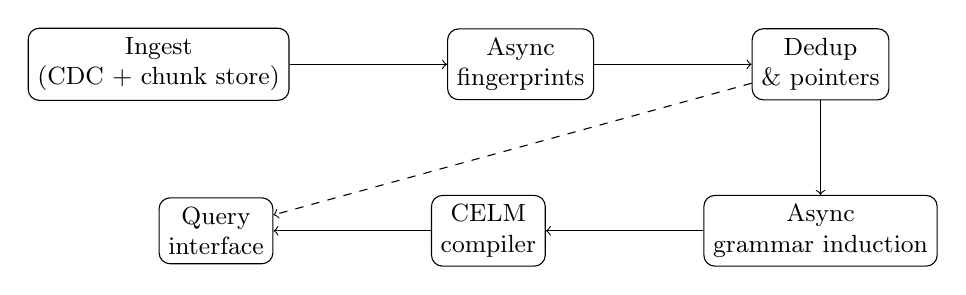
\begin{tikzpicture}[node distance=1.25cm, every node/.style={font=\small}]
\node[draw,rounded corners,align=center] (ingest) {Ingest\\(CDC + chunk store)};
\node[draw,rounded corners,align=center,right=2.0cm of ingest] (fp) {Async\\fingerprints};
\node[draw,rounded corners,align=center,right=2.0cm of fp] (dedup) {Dedup\\\& pointers};
\node[draw,rounded corners,align=center,below=1.2cm of dedup] (grammar) {Async\\grammar induction};
\node[draw,rounded corners,align=center,left=2.0cm of grammar] (compile) {CELM\\compiler};
\node[draw,rounded corners,align=center,left=2.0cm of compile] (query) {Query\\interface};

\draw[->] (ingest) -- (fp);
\draw[->] (fp) -- (dedup);
\draw[->] (dedup) -- (grammar);
\draw[->] (grammar) -- (compile);
\draw[->] (compile) -- (query);
\draw[->,dashed] (dedup) -- (query);
\end{tikzpicture}
\caption{High-level pipeline: synchronous ingest, asynchronous enrichment, and snapshot-based CELM compilation.}
\label{fig:pipeline_overview}
\end{figure}

\section{Retrieval Output Contract}
The analysis interface is designed around traceability. Given an input string $s$, the system returns:
\begin{itemize}
  \item \textbf{Normalised query representation} (tokenisation and canonicalisation decisions, including the data programming rules that were applied).
  \item \textbf{Candidate chunk matches} with similarity scores and the fingerprints that triggered each candidate (exact hash hit, MinHash/SimHash similarity, token-level matches, etc.).
  \item \textbf{Context windows} via follow pointers: predecessor and successor chunks, including aggregated statistics such as average out-degree (follow pointers) and in-degree (inbound references).
  \item \textbf{Grammar explanation} where available: the rules/non-terminals that cover the matched region and how they expand back to observed chunks.
  \item \textbf{Operational metrics} such as latency, index probe counts, and cache hit rates.
\end{itemize}

\noindent This contract differs from typical LLM inference: instead of returning a sampled continuation, the system returns a traceable \emph{programmatic explanation} of how a result was assembled from stored evidence.

\section{Storage Interfaces}
ComdareDB supports multiple storage interfaces (file-based, archive-based, and future network-based interfaces). Interfaces share a common ingestion core (chunking + metadata extraction) so that fingerprint and grammar learning remain consistent across domains.

\section{What CELM Produces}
The compilation target is a binary artifact that bundles:
\begin{itemize}
  \item a compact representation of grammar rules and non-terminals,
  \item fingerprint postings needed for query-time matching,
  \item pointer graph summaries (to reconstruct context windows),
  \item and an execution entry point implementing the retrieval output contract.
\end{itemize}

\noindent The resulting ``model'' is therefore closer to a specialised retrieval-and-compilation engine than to a generative transformer. This is intentional: the focus is traceability and efficient reuse of previously seen information.
\chapter{Evaluation Plan}
A full benchmarking campaign is planned as a follow-up iteration. This chapter defines the evaluation dimensions and the metrics that will be used to assess ComdareDB and CELM.

\section{Evaluation Dimensions}
We separate evaluation into three dimensions:
\begin{enumerate}[label=\textbf{D\arabic*.},leftmargin=1.4cm]
  \item \textbf{Storage and Deduplication Efficiency.} How much physical storage is saved, and what overhead does indexing introduce?
  \item \textbf{Pipeline and System Performance.} Can ingestion remain fast while asynchronous jobs run, and what are the latency/throughput characteristics of query execution?
  \item \textbf{Compilation and Output Quality.} Does CELM provide useful, traceable results and stable behaviour across snapshots?
\end{enumerate}

\section{Metrics}
\subsection{Deduplication and Graph Metrics}
The following metrics are adopted from deduplication-oriented database analysis and are directly applicable to ComdareDB's chunk graph:

\begin{itemize}
  \item \textbf{Deduplication ratio (DR).} Defined as $\text{logical\_bytes} / \text{physical\_bytes}$ (or equivalently, the percentage saved). This is a standard storage deduplication metric \cite{Muthitacharoen2001,Quinlan2002}.
  \item \textbf{Average follow-pointer out-degree.} Average number of successor links per chunk (context fan-out). High values indicate branching contexts.
  \item \textbf{Average inbound-pointer in-degree.} Average number of references to a chunk from other chunks (reuse fan-in). High values indicate strong deduplication and structural sharing.
  \item \textbf{Chunk fan-out distribution.} Distribution (mean/median/p95) of follow pointers, to detect hotspots and skew.
\end{itemize}

\subsection{Indexing and Write Amplification Metrics}
Inline deduplication and fingerprint indexing introduce write overhead. We track:

\begin{itemize}
  \item \textbf{Index write amplification.} Bytes written to indexes (posting lists, metadata, grammar store) per ingested byte. This metric is closely related to write amplification in LSM-style systems \cite{ONeil1996,Dayan2017}.
  \item \textbf{Update amplification under merge.} Additional index updates caused by deduplication merges and graph repair.
\end{itemize}

\subsection{Performance Metrics}
\begin{itemize}
  \item \textbf{Ingest throughput.} Sustained input rate (bytes/s) while background jobs are active.
  \item \textbf{Query throughput.} Queries/s for the analysis interface under controlled workloads.
  \item \textbf{Latency.} End-to-end latency distributions (p50/p95/p99) for ingest and query.
  \item \textbf{Background job backlog.} Queue depth and time-to-completion for fingerprint and grammar jobs (measures how well async processing keeps up).
\end{itemize}

\subsection{Compilation and Output Quality Metrics}
Because CELM aims for traceable program output, quality is evaluated via:
\begin{itemize}
  \item \textbf{Trace completeness.} Fraction of output items that can be linked back to concrete chunks and grammar rules.
  \item \textbf{Stability across snapshots.} How much does the CELM output change when new data is ingested (measured by diffing traces).
  \item \textbf{Retrieval quality.} Precision/recall-like measures on curated query sets (optional, future iteration).
\end{itemize}

\section{Baselines and Comparisons}
The initial baseline set targets comparable storage and indexing systems:

\begin{itemize}
  \item \emph{LSM-based key-value stores} (e.g., RocksDB as a reference for write amplification and throughput characteristics) \cite{ONeil1996,Dayan2017}.
  \item \emph{Content-addressed archival storage} such as Venti \cite{Quinlan2002}.
  \item \emph{CDC-based deduplication systems} such as LBFS-style chunk stores \cite{Muthitacharoen2001,Xia2016}.
\end{itemize}

\noindent In addition, we compare the \emph{output contract} to classical retrieval pipelines (keyword search and embedding-based retrieval) and to transformer LLMs with RAG \cite{Lewis2020}. This comparison is conceptual at this stage and will be quantified in later iterations.
\chapter{Expected Results and Discussion of Limitations}
\section{Expected Results}
The expected outcome of this work is a clearer architectural argument for why a database-centric pipeline can serve as a compiler front-end for language modelling.

On the storage side, ComdareDB is expected to achieve competitive deduplication ratios on mixed datasets by combining CDC chunking with multi-fingerprint similarity search. On the modelling side, CELM is expected to produce \textbf{traceable program output}: results that explicitly reference stored chunks, pointer graph links, and grammar rules. This traceability is the core differentiator compared to transformer-based LLM inference, where intermediate structure is not explicitly represented.

\section{Limitations and Risks}
Several limitations are inherent to the approach:

\begin{itemize}
  \item \textbf{Expressiveness vs. feasibility.} Grammar induction algorithms are typically context-free approximations and may miss genuinely context-sensitive dependencies. ComdareDB can approximate context sensitivity via pointer graph conditioning and multi-fingerprint evidence, but this is not equivalent to full Type-1 grammar learning.
  \item \textbf{Complexity of grammar learning.} Even practical algorithms such as Sequitur/Re-Pair introduce computational overhead, and care is required to keep asynchronous job backlogs under control.
  \item \textbf{Not a general-purpose chatbot.} CELM is not designed to replace state-of-the-art transformer LLMs for open-ended generation. The target is retrieval, compilation, and explanation over the database's own content.
  \item \textbf{Evaluation deferred.} This iteration establishes architecture and metric definitions; quantitative benchmarks and end-to-end quality evaluation require a dedicated follow-up.
\end{itemize}

\noindent These limitations are acceptable given the stated scope: the goal is to make the internal database mechanics understandable and to show a plausible path from deduplication metrics and inferred grammars to a compilable, executable model artifact.
\chapter{Conclusion and Outlook}
This report presented ComdareDB as a database substrate for Eigentokens and CELM compilation. The central idea is to treat deduplication, multi-fingerprint equivalence, and inferred grammars as a compilation-grade intermediate representation: a database snapshot can be compiled into a deterministic, executable artifact that provides traceable program output.

\textbf{RQ1 (compilability and use of a model artifact)} is addressed by specifying CELM as a concrete compilation target with an explicit output contract, and by outlining a snapshot-based compilation pipeline that decouples ingestion from analysis via asynchronous jobs.

\textbf{RQ2 (grammar and grammar learning)} is addressed by grounding the work in the Chomsky hierarchy, by relating grammar induction algorithms (Sequitur/Re-Pair style) to practical structure discovery, and by showing how context signals can be approximated through a pointer graph and multi-fingerprint evidence.

\section{Outlook}
The next iterations of this project should focus on:
\begin{itemize}
  \item implementing and reporting the benchmark suite described in Chapter~7 (deduplication ratio, pointer graph statistics, index write amplification, throughput, latency),
  \item analysing the sensitivity of grammar hypotheses to noisy or adversarial inputs,
  \item and evaluating how CELM can interoperate with transformer LLMs (e.g., as a grounding/retrieval component).
\end{itemize}

\noindent A longer-term follow-up question connects this work to autonomous systems research:

\begin{quote}
Is it possible to build a system that autonomously adapts to the requirements of a given task and its environment, and that can compile AI models on-demand (for a given topic) into its own binary programs?
\end{quote}

\noindent ComdareDB and CELM provide a first building block for such a system: they define a deterministic compilation target and an asynchronous pipeline that turns stored knowledge into executable artifacts. Autonomy would additionally require capability discovery, resource-aware scheduling, and safe sandboxing of dynamically compiled components.

\appendix
\chapter{Prototype Implementation Snapshot}
This appendix summarises implementation-oriented aspects of the proof-of-concept. The main body focuses on \emph{what} is built and \emph{why}; this appendix captures \emph{how much} and \emph{where} without turning the report into a code catalogue.

\section{Key Modules (Conceptual)}
The prototype is organised into a small set of conceptual modules:
\begin{itemize}
  \item \textbf{Chunk store / TreeCore:} chunk persistence and pointer graph maintenance.
  \item \textbf{Fingerprint core:} computation and storage of exact, rolling, and approximate fingerprints.
  \item \textbf{Async pipeline:} scheduler, job queues, and idempotent workers for fingerprint expansion, merge decisions, and grammar induction.
  \item \textbf{Grammar store:} persistent representation of inferred rules and non-terminals.
  \item \textbf{Compiler:} snapshot selection and CELM artifact emission.
  \item \textbf{Interfaces:} storage adapters (files/archives) and analysis/query interface.
\end{itemize}

\section{Why the Implementation is Split}
The database is intentionally modular to allow experimentation with fingerprint families, storage backends, and compilation strategies. This modularity is reflected in a set of linked repositories and generic modules; detailed inventory data is maintained in internal project documentation \cite{ComdareDBFeatureCatalog2026,HauntedRequest9}.

\end{document}
